\section{Material and Methods} \label{matmet}

\subsection{Data acquisition}
%~ 
In this study, 12 male mice (Tg(Gal-cre)KI87Gsat/Mmucd, FVB/N-Crl:CD1(ICR) hybrid strain),
between 8 and 12 week old were used.
Animal were housed under a 12h light/dark light cycle.
Small (diam. = 1mm) holes were drilled in the scull of anaesthetised animals.
For the  \gls{eeg}, the reference-ground electrode was placed into the parietal bone (Bregma -1.5, mediolateral (ML) +1.5) and
 the other electrode was placed into the frontal bone (Bregma +1.5, ML -1.5).
For \gls{emg} acquisition, three polytetrafluoroethylene-insulated stainless steel electrodes were placed into the neck muscles.

Both signals were recorded by a miniature
`neurologger'\cite{vyssotski_miniature_2006}.
The recording device applies band-pass analogue filtering between 1 and 70Hz and converts both analogue signals to digital time series at a sampling rate of approximately 200.0Hz.
All 12 animals were monitored for approximately 24h.

Sleep scoring was performed in a semi-automatic fashion by a trained
expert.
A first, human assisted, pass was applied to generate preliminary annotations on the basis of logical rules\cite{costa-miserachs_automated_2003}.
Then, the expert visually inspected and, when required, corrected the annotations.
Annotation were generated for consecutive epochs of approximately 5.0s.

Data acquisition and manual annotation were performed by Dr. Valentina
Ferretti and Eleonora Steinberg prior to this project.
%~ 
\subsection{Data preprocessing}

\gls{eeg} and \gls{emg} signals were resampled from approximately 200.0Hz to 256.0Hz using
conservative sinc interpolation\cite{putnam_design_1997}.
A sampling frequency of $f_s  = 256.0$Hz is convenient since is implies that discrete wavelet decomposition (see subsection~\ref{sub:features} and fig.~\ref{fig:dwd}) will separate
frequencies above 4.0Hz from those below 4.0Hz (since $4 = 256.0/{2^6} $).
This frequency is typically uses as a cut-off value between theta and delta
waves \cite{vyazovskiy_nrem_2014}.
In addition, \gls{eeg} and \gls{emg} signals were standardised ($E[x] = 0, Var[x] = 1$) to account for the variability in baseline amplitude due to acquisition.
Vigilance state annotations were resampled at exactly 0.20Hz using nearest neighbour interpolation.

\subsection{Feature extraction from time series}
\label{sub:features}

A wavelet transform based feature extraction strategy was adopted.
In summary, discrete wavelet decomposition was used on both \gls{eeg} and \gls{emg}
in order to separate frequency bands (fig.~\ref{fig:dwd}).

\begin{figure}[h!]
  \centering   
    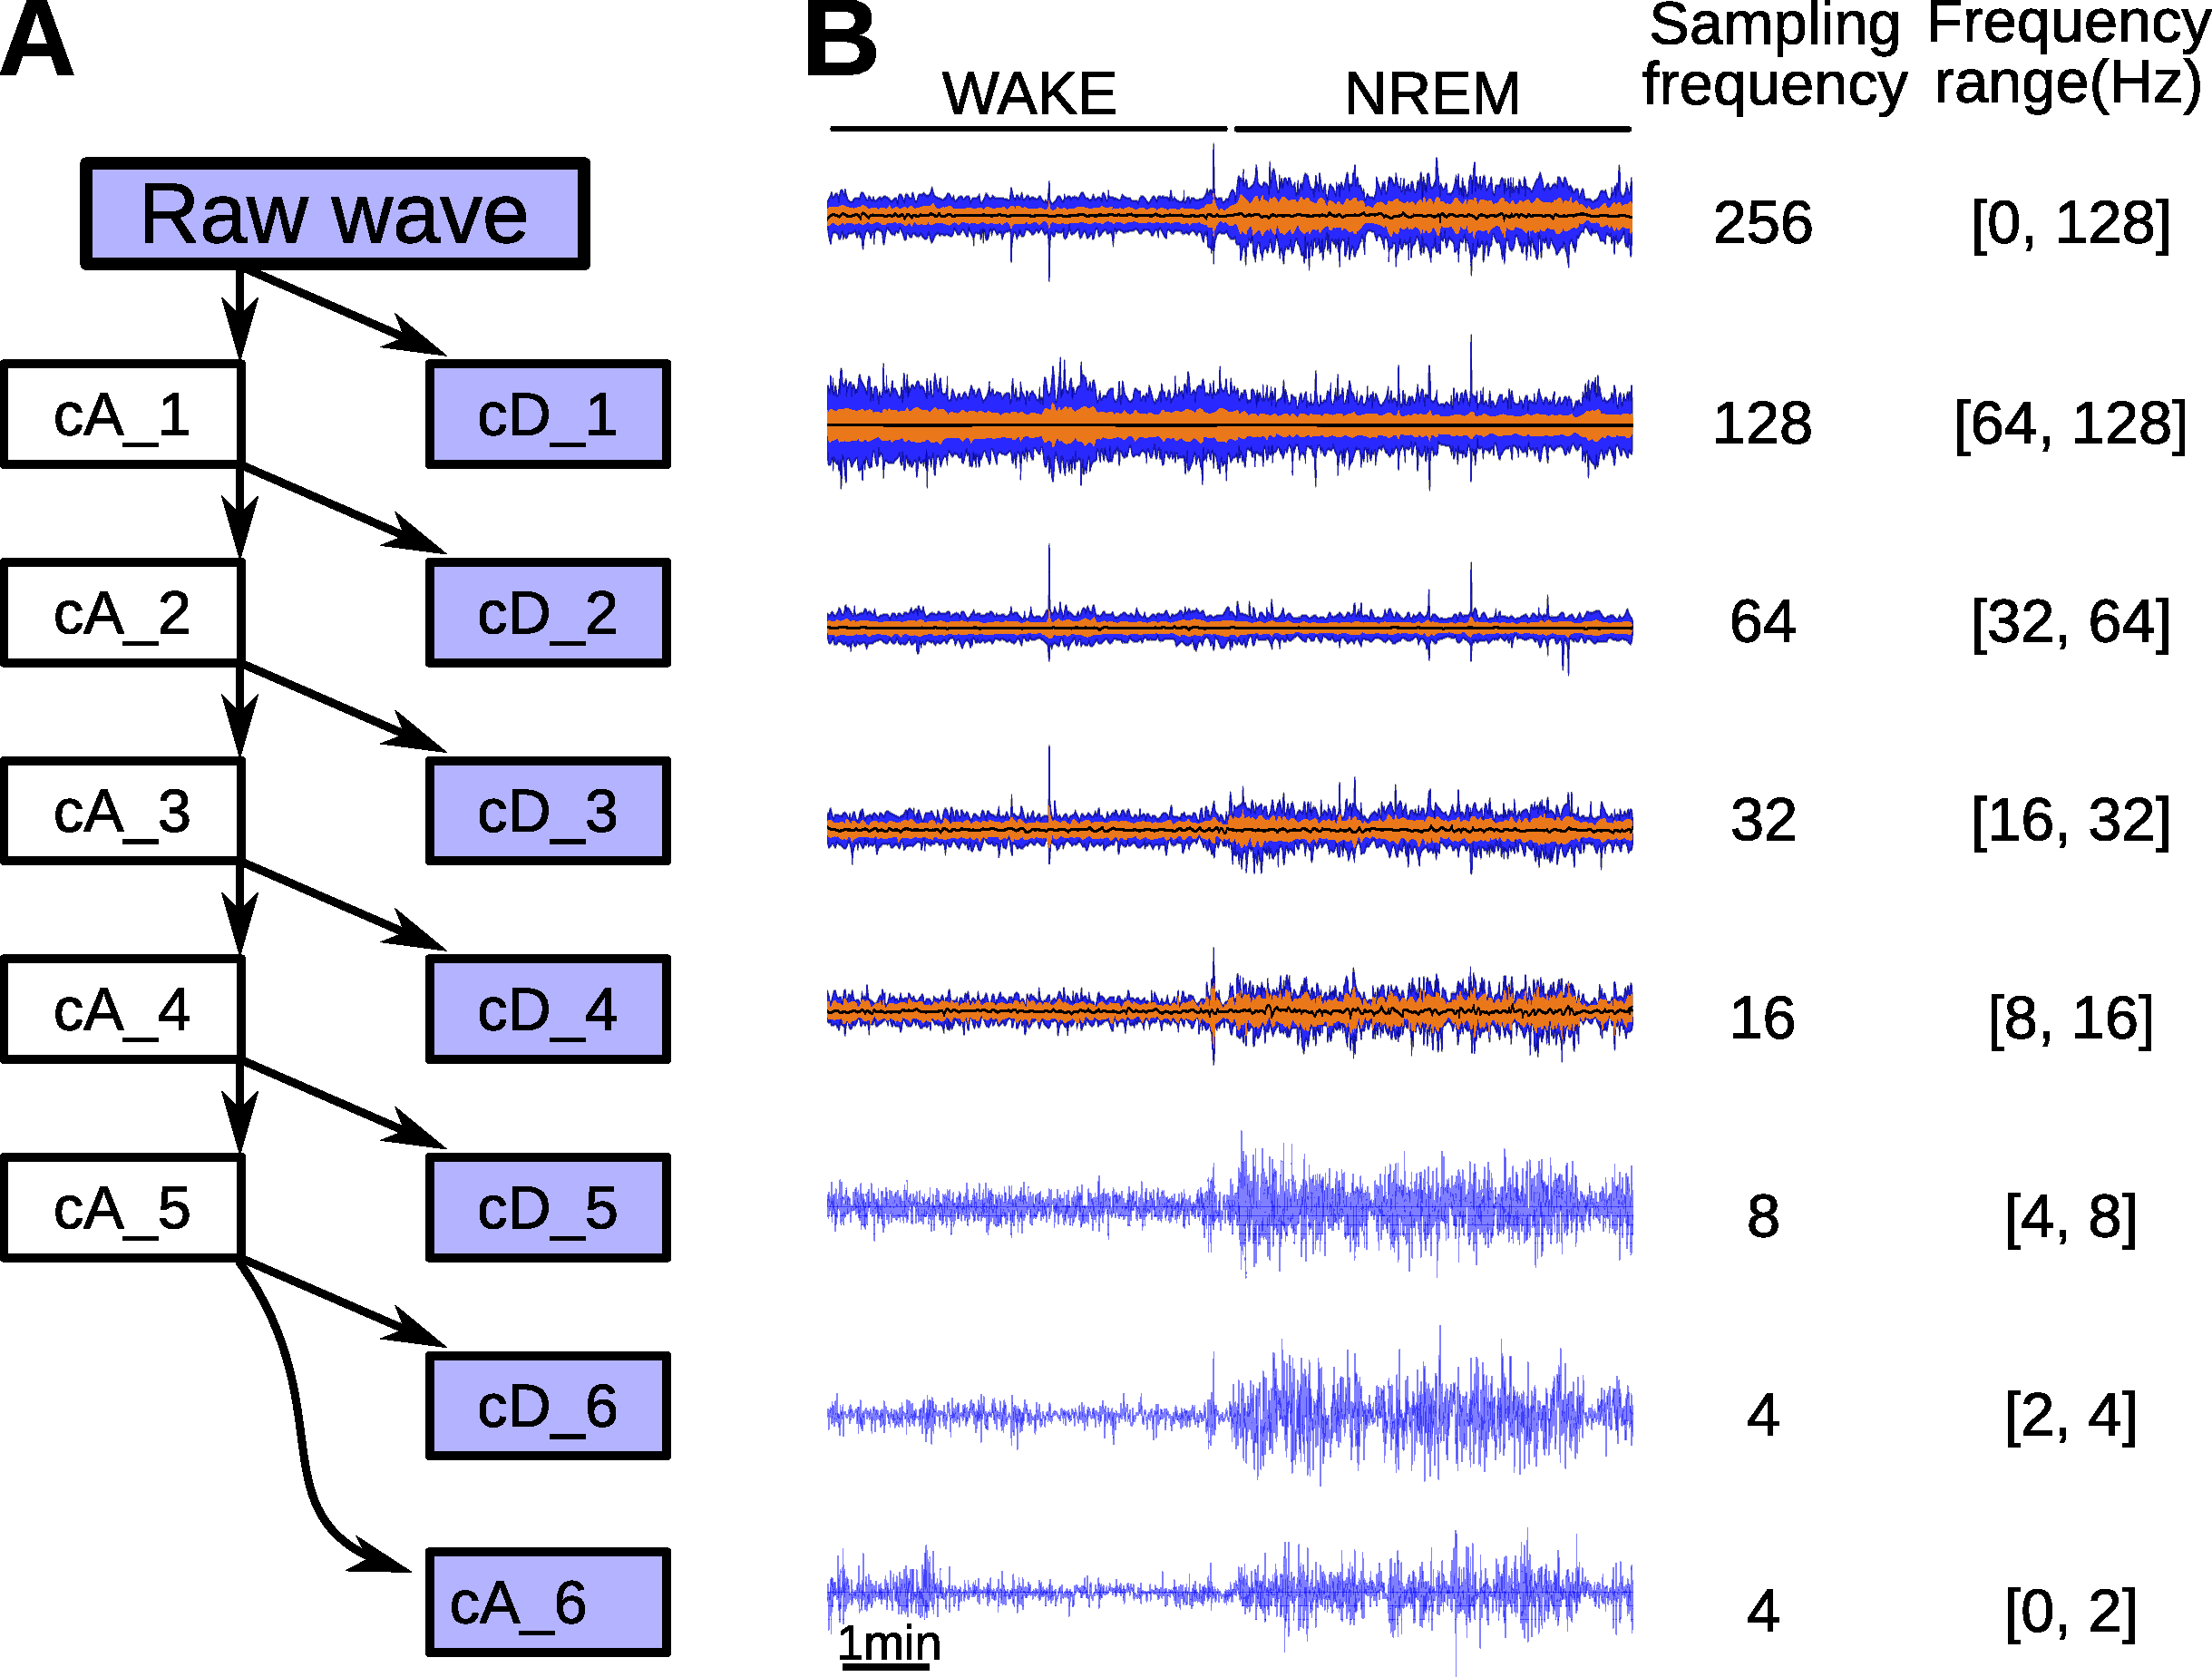
\includegraphics[width=0.95\textwidth]{figures/dwd.pdf}
  \caption{\ctit{Discrete wavelet decomposition.}
	\textbf{A}, Through discrete wavelet transform the initial signal is split into a pair of coefficients: $cA$ and $cD$, which capture the low ($[0, f_s/2]$), and high $[f_s/2, f_s]$ frequency information, respectively.
	Then, discrete wavelet transform is applied iteratively on subsequent $cA$ coefficients ($cA\_1, ..., cA\_n$), thus generating ($cD\_1, ..., cD\_n$).
	In this example, decomposition is performed up to the sixth level ($n=6$).
	\textbf{B}, 
	Ten minutes representing the \gls{eeg} of a transition between a wake and a slow wave sleep(NREM) are shown for the raw
	 wave and for each of the coefficients that are kept for feature extraction (blue rectangles in A).
	 The variation of amplitude in each coefficient corresponds to a concomitant variation of amplitude in the frequency range of this coefficient.
	 In this example, the general increase in power in the raw wave corresponds to an increase of power in the frequency bands below 32Hz, but with a decrease in power above 64Hz.
	%~ Later, each of the eight time series will be segmented into five second epochs, and features are computed for all epochs in the wavelet coefficients and the  raw signal.
	In this figure, the five first signals are too dense to be rendered in a usual fashion. Instead, only local range(blue), inter-quantile range (orange) and median (black line) are represented.
  \label{fig:dwd}
  }
\end{figure}







Discrete wavelet decomposition was applied \emph{a priori} to the whole signals
in order to avoid edge effects (see \cite{prabhakar_application_2002} for a
simple application of discrete wavelet on digital signals).
The maximum decomposition levels for the \gls{eeg} and \gls{emg} signals were six and four, respectively.
Daubechies wavelet, with four vanishing moments (``db4'') was used.
As a result, a total of 14 time series was generated for each recording.

For all time series, a list of 16 features (see table~\ref{tab:features}) was computed in each subsequent non-overlapping five seconds epochs.
Thus, resulting in a total of $p=192$ variables. 
For each recording ($\simeq 24h$) there were approximately $17000$ epochs.
Some combinations of variables and signals were however incalculable.
These were therefore removed; resulting in an actual number of variables $p=164$.



\begin {table}[!h]
\begin{center}
\caption{\ctit{List of features.}
For clarity, features were classified in four functionnal families.
16 scalar features, in four families, are computed for each epoch.
Since all features are computed for all wavelet coefficients and raw signals (\gls{eeg} and \gls{emg}), a total of 
$16 \times (1+7 + 1 + 3) = 192$ features are generated every five second of recording.
The mathematical detail of the algorithms is provided in the documentation of \pr{} (see appendix).
\label{tab:features}}

\small
\begin{tabular}{|c|c|}
  \hline
  Feature family & features\\
 \hline
 \hline
  Power & \specialcell{\texttt{mean}, \texttt{sd}, \texttt{skewness}, \texttt{kurtosis}\\\texttt{median}, \texttt{min}, \texttt{max}}\\
  \hline
  Hjorth & \texttt{morbidity}, \texttt{complexity}\\
  \hline
  Fractal & \texttt{Petrosian} and \texttt{Higuchi} fractal dimensions\\
  \hline
  Entropy & \specialcell{\texttt{Fisher information}, \texttt{SVD entropy}\\and \texttt{Sample entropy} with $m=2$, and $ r \in \{ 0.2, 1.0, 1.5\}$}\\
 \hline



\end{tabular}
\end{center}
\end{table}



Features were extracted using, \pr{}, a \py{} package developed as part of this project.


\subsection{Addition of temporal features}
Two strategies, ``lag'' and ``convolution'', were used to add temporal
information to the variable space\cite{dietterich_machine_2002}.
For lag, given a vector $\mathbf{X_t}$ of feature at time $t$,
A new vector of feature was defined as $\mathbf{{X'}_t}$ as
\begin{equation}
\mathbf{{X'}_t} = \{\mathbf{X_{t-\tau}}, ..., \mathbf{X_t}, ..., \mathbf{X_{t+\tau}}\}
\label{eq:tau}
\end{equation}
with $\tau \in \mathbb{N}$.

For convolution, the local average $\mathbf{W^n_t}$ of each variable over several rectangular windows of sizes $n$ was added:
\begin{equation}
\mathbf{{X'}_t} = \{W^{n_1}_t, W^{n_2}_t, ...\}
\label{eq:window}
\end{equation}
where
\[
\mathbf{W^n_t} = \frac{1}{2n+1} \sum_{i = t-n}^{t+n}{X_i}
\]
and $n$ is a set of odd integers representing window sizes (\eg $\{1,3,7,15\}$).



\subsection{Stratified Cross Validation and sampling}


Stratified cross-validation was systematically applied to generate vigilance state predictions.
That is, in order to generate prediction for a given time series, classifiers were always trained with a subsample of epochs
originating from all \emph{other} time series \cite{ding_querying_2008}.

Quantification of variable importance and accuracy (figs.~\ref{fig:variable_elimination} and ~\ref{fig:temporal_integration}) was performed in order 
not to underestimate the relevance of the minority class
(\gls{rem})\cite{boulesteix_overview_2012}.
Class  unbalancedness was accounted for by fitting predictors on balanced subsamples (750 epochs of each class per tree).


\subsection{Random forests analysis}
Unless specified otherwise, random forests\cite{breiman_random_2001}were trained
with balanced samples of 1000 epochs per class.
In order to select variables and define new features, forests with 50 classification trees were built.
100 trees were used otherwise.
Increasing the sample size and number of trees did not seem to improve performance.
The number of variables drawn for each split, $mtry$, was set to the default value for classification problems $\sqrt{p}$.
Variable importance was assessed by the average (over all trees) decrease in Gini impurity induced by a given variable.
All random forest analysis was implemented in \texttt{R} statistical software
\cite{r_core_team_r:_2014}, using the package
\texttt{randomForest}\cite{liaw_classification_2002}.

To produce an overall summary value of confidence, an entropy based metric $c$ was defined as:
\begin{equation}
c = 1 + \frac{1}{log_2(k)}\sum{v_i  log_2(v_i)}
\label{eq:entropy}
\end{equation}
where $v_i$ is the proportion of votes for the class $i$, and $k$ is the number of classes. 
This definition has the following properties 
\[
c \in [0;1]
\]
\[
v_1 = v_2 = ... = v_k \rightarrow c = 0
\]
\[
v_i = 1 \rightarrow c = 1 , \forall i
\]




\subsection{Performance assessments}
Comparisons of runtime between \pr{} and \pyeeg{}\cite{bao_pyeeg:_2011} were performed by
measuring the average (between 2 and 100 run, depending on the algorithm) runtime of algorithms on six normally distributed ($\mathcal{N}(\mu=0,\sigma=1)$) random time series (\ie{} white noise) of size $n$,
with $n$ between $256 \times{} 5$ and $256 \times{} 30$.
This was repeated five times for each time series.
For computing  Higuchi fractal dimension\cite{higuchi_approach_1988}, $k_{max}$
was set to $2^3$.
For both approximate entropy and sample
entropy\cite{richman_physiological_2000}, the embedding dimension $m$ was set to $2$, and the distance threshold, $r$, to $1.5$.
For fisher information, the embedding dimension and the delay, $\tau$ were set to $3$ and $2$, respectively.
Finally, spectral entropy was computed for the frequency bands bounded by $\{0, 2^0, 2^1, ..., 2^6\}$Hz, with $f_s = 256.0$.
Benchmarks were generated using \texttt{CPython 2.7.8} on \texttt{GNU/Linux} operating stystem with a 3.40GHz intel i7-3770 CPU.

\subsection{Statistical analysis}
In order to test significance in the difference of performance between \pr{} and \pyeeg{} (table~\ref{tab:benchmark}),
linear models were fitted on the log-transformed runtime for each algorithm. 
t-tests on the effect of the implementation (\ie{} whether \pr{} or \pyeeg{} was used) on the intercept at $x=1280$, were used to compute $p-values$ at $n=1280$.
Significance levels for the differences in scaling were obtained through t-tests on the interaction between $n$ and the implementation.


In order to assess the significance of the effect of the addition of temporal variables on the cross-validation
error (fig.~\ref{fig:temporal_integration}), repeated t-tests were performed.
Bonferronni correction was applied.

In order to determine whether state prevalences were different between predicted and ground truth time series (fig.~\ref{fig:struct_assess}A),
beta regression \cite{cribari-neto_beta_2009} was fitted. 
Then, interactions between state and method (\ie{} prediction vs. ground truth) were tested with a z-test.

In order to determine the effect of prediction on the number of episodes of each state (fig.~\ref{fig:struct_assess}B),
Poisson generalised linear mixed model, using recordings (\ie{} animals) as a
random effect, was fitted using \texttt{lme4}\cite{bates_lme4:_2014}.
Then, interaction between state and method were tested with a t-test.

Finall, in order to determine the effect of prediction on the average duration of episodes of each state (fig.~\ref{fig:struct_assess}B),
linear mixed model on log-transformed duration, using recordings (\ie{} animals) as a random effect, was fitted. 
Then, interaction between state and method were tested with a t-test.

All statistical analysis were performed with \texttt{R}
software \cite{r_core_team_r:_2014}.
%~ 
